\section{Results}
\subsection{Spectra Clusterization}
Clusterization of spectra will be presented using data gathered on ``Portrait of John III Sobieski in Karacena Scale Armour'' (see \prettyref{fig:sobieski_fragment}).
\begin{figure}[H] 
  \centering     
  \includegraphics[width=0.5\textwidth]{img/jan_sobieski_w_karacenie.png} 
  \caption{An examined fragment of ``Portrait of John III Sobieski in Karacena Scale Armour''. Source: \cite{wikimediaSobieskiPortrai} }
  \label{fig:sobieski_fragment}
\end{figure}

\subsubsection{Clusterization With SOM}
The first clustering algorithm, SOM, was invoked as presented in \prettyref{lst:som-invocation}.
\newenvironment{longlistingG}{\captionsetup{type=listing, width=0.8\textwidth}}{}
\begin{longlistingG}
    \pythoncode{listings/som_invocation.py}
    \caption{Invocation of SOM algorithm}
    \label{lst:som-invocation}
\end{longlistingG}
\vspace{12pt}

The arguments used to initialize \texttt{SelfOrganizingMap} are:
\begin{description}
    \item[\texttt{input\_size}:] Configured to the number of channels (4094 in this instance).
    \item[\texttt{map\_size}:] Set to (3, 3), indicating a total of $3 \times 3 = 9$ clusters.
    \item[\texttt{learning\_rate}:] The learning rate during the first epoch.
    \item[\texttt{sigma\_neigh}:] The influence on the neighbors of the BMU. Lower values result in larger influence.
    \item[\texttt{sigma\_decay}:] The rate of decay for the learning rate. Lower values result in slower decay.
\end{description}
The performance of the algorithm scales linearly with the number of clusters. 
With a total of 9 clusters, the clusterization of data with shape of (524, 348, 4094) takes approximately 6 minutes. 
Therefore, it may not be feasible method if many more clusters were needed, at least while using basic python implementation and performing clusterization globally.

The result of applying clusterization on raw spectrum can be observed on \prettyref{fig:sobieski_clustered_som_noise}.

\newpage
\begin{figure}[H] 
  \centering     
  \includesvg[width=1\textwidth]{img/sobieski_clustered_som_noise.svg} 
  \caption{Clusterization of unprocessed spectrum of ``Portrait of John III Sobieski in Karacena Scale Armour'' using SOM}
  \label{fig:sobieski_clustered_som_noise}
\end{figure}

As the reader may notice, certain clusters are artificial. 
It was sensible to investigate the possibility of the artifacts arising from a poor implementation of the SOM algorithm.
This involved employing a UMAP to HDBSCAN pipeline to validate the clustering results.

\subsubsection{Clusterization With UMAP And HDBSCAN}
Clusterization with UMAP and HDBSCAN was invoked as presented in \prettyref{lst:umap-hdbscan-invocation}.

\newenvironment{longlistingH}{\captionsetup{type=listing, width=0.8\textwidth}}{}
\begin{longlistingH}
    \pythoncode{listings/umap_hdbscan_invocation.py}
    \caption{Invocation of UMAP to HDBSCAN pipeline}
    \label{lst:umap-hdbscan-invocation}
\end{longlistingH}
\vspace{12pt}

The meaning of arguments passed to UMAP is as follows:
\begin{description}
    \item[\texttt{n\_neighbors:}] The number of neighbors used for manifold approximation. As \texttt{n\_neighbors} increases more focus is placed on the global structure of the data. 
    \item[\texttt{min\_dist:}] The minimum distance between points in the dimensional embedding. For clusterization, values around 0 are preferred, because it is desirable to transform data into "tightly packed" clumps.
    \item[\texttt{n\_components:}] The number of dimensions in the low-dimensional representation. Experimentation showed that reducing dimensions to one gave the best results. 
\end{description}

Arguments for HDBSCAN are:
\begin{description}
    \item[\texttt{min\_samples:}] The number of samples in a neighborhood for a point to be considered a core point.
    \item[\texttt{min\_cluster\_size:}] The minimum number of points required to form a cluster. It is probably the most important parameter; smaller values will lead to more clusters.
    \item[\texttt{metric:}] The distance metric used for clustering. Euclidean distance works well, although other popular metrics give good results too.
\end{description}

Dimensionality reduction using UMAP took approximately 7 minutes. 
The cost scales with the parameter \texttt{n\_neighbors}.
Further clusterization with HDBSCAN is much faster (due to the really low dimensionality of input) and allows for fast experiments with different parameters, e.g. to achieve the desired granularity of clusters.

It appears that although clusterization worked, it did not prevented artifacts from appearing - see \prettyref{fig:sobieski_clustered_hdbscan_noise}.
\begin{figure}[H] 
  \centering     
  \includesvg[width=1\textwidth]{img/sobieski_clustered_hdbscan_noise.svg} 
  \caption{Clusterization of unprocessed spectrum of ``Portrait of John III Sobieski in Karacena Scale Armour'' using UMAP and HDBSCAN}
  \label{fig:sobieski_clustered_hdbscan_noise}
\end{figure}

\newpage
\subsubsection{Source of Clusterization Artifacts}
The source of clusterization artifacts remains unknown as of today. 
However, due to the nature of the artifacts, they may be attributed to a poorly implemented pinhole camera.
Two possible implementations of a pinhole camera are demonstrated in \prettyref{fig:pinhole-camera-implementations}.

\begin{figure}[H]
  \centering
  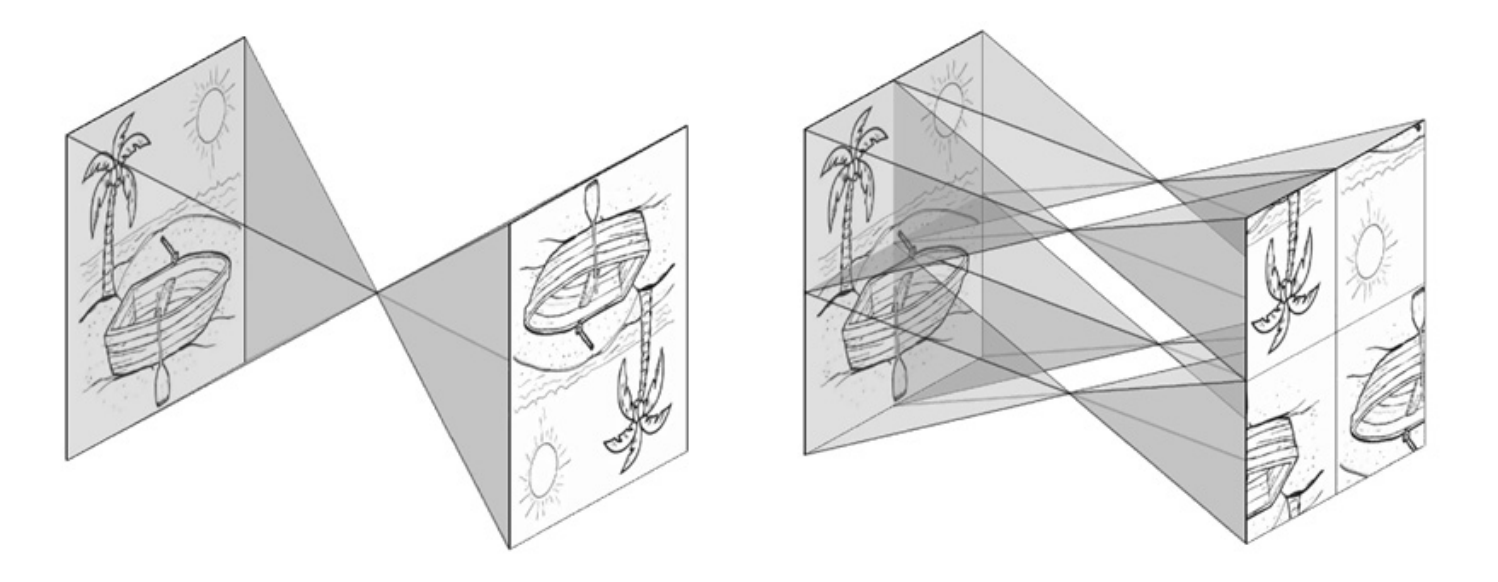
\includegraphics[width=0.8\textwidth]{img/pinhole_camera.png}
  \caption{1-hole pinhole camera (left) and 4-hole pinhole camera (right). Source: \cite{Lach2022}}
  \label{fig:pinhole-camera-implementations}
\end{figure}

The details of the pinhole camera implementation used during measurements are unknown, but the artifacts strongly suggest that a 4-hole pinhole camera was used. 
It seems that differences between pinhole cameras lead to different artifacts showing up during clusterization. 
Fortunately, the clusterization problem turned out to be easily solvable.

\newpage
\subsubsection{Clusterization Results}
By simply removing one hundred points from both ends of the spectrum, the results of clusterization were tremendously improved, as visible in \prettyref{fig:som-clusterization-clean} and \prettyref{fig:hdbscan-clusterization-clean}.

\begin{figure}[H]
  \centering
  \includesvg[width=1\textwidth]{img/sobieski_clustered_som_clean.svg}
  \caption{Clusterization of the cropped spectrum of ``Portrait of John III Sobieski in Karacena Scale Armour'' using SOM.}
  \label{fig:som-clusterization-clean}
\end{figure}

\begin{figure}[H]
  \centering
  \includesvg[width=1\textwidth]{img/sobieski_clustered_hdbscan_clean.svg}
  \caption{Clusterization of the cropped spectrum of ``Portrait of John III Sobieski in Karacena Scale Armour'' using UMAP and HDBSCAN.}
  \label{fig:hdbscan-clusterization-clean}
\end{figure}

\newpage
To better understand the clusters they can be visualized on separate pictures, as shown in \prettyref{fig:som-clusters-clean} and \prettyref{fig:hdbscan-clusters-clean}.
\begin{figure}[!htbp]
  \centering
  \includesvg[width=0.8\textwidth]{img/sobieski_clusters_som_clean.svg}
  \caption{Separate clusters from SOM clusterization}
  \label{fig:som-clusters-clean}
\end{figure}

\begin{figure}[!htbp]
  \centering
  \includesvg[width=0.8\textwidth]{img/sobieski_clusters_hdbscan_clean.svg}
  \caption{Separate clusters from UMAP and HDBSCAN clusterization}
  \label{fig:hdbscan-clusters-clean}
\end{figure}


\newpage
\label{sec:clustered-spectra}
Spectra from each cluster were accumulated and preprocessed (as was discussed in \prettyref{sec:data-preprocessing}) before being passed to classifier - see \prettyref{fig:som-spectra} and \prettyref{fig:hdbscan-spectra}.

\begin{figure}[!htbp]
  \centering
  \includesvg[width=1\textwidth]{img/sobieski_spectra_som_clean.svg}
  \caption{Processed spectra from SOM clusterization}
  \label{fig:som-spectra}
\end{figure}

\begin{figure}[!htbp]
  \centering
  \includesvg[width=1\textwidth]{img/sobieski_spectra_hdbscan_clean.svg}
  \caption{Processed spectra from UMAP and HDBSCAN clusterization}
  \label{fig:hdbscan-spectra}
\end{figure}